\chapter{Frontend}
    Questa parte dell'applicazione consiste in un'interfaccia grafica che consente all'utente di visualizzare, sostituire i test e di committarne le modifiche.\\
    Pu\'o anche essere integrata con un tool esterno per consultare le differenze tra il risultato atteso e quello ottenuto nei test in errore.\\
    L'interfaccia \'e una pagina web dinamica perciò disponibile online a tutti gli sviluppatori.\\
    \begin{figure}[h]
        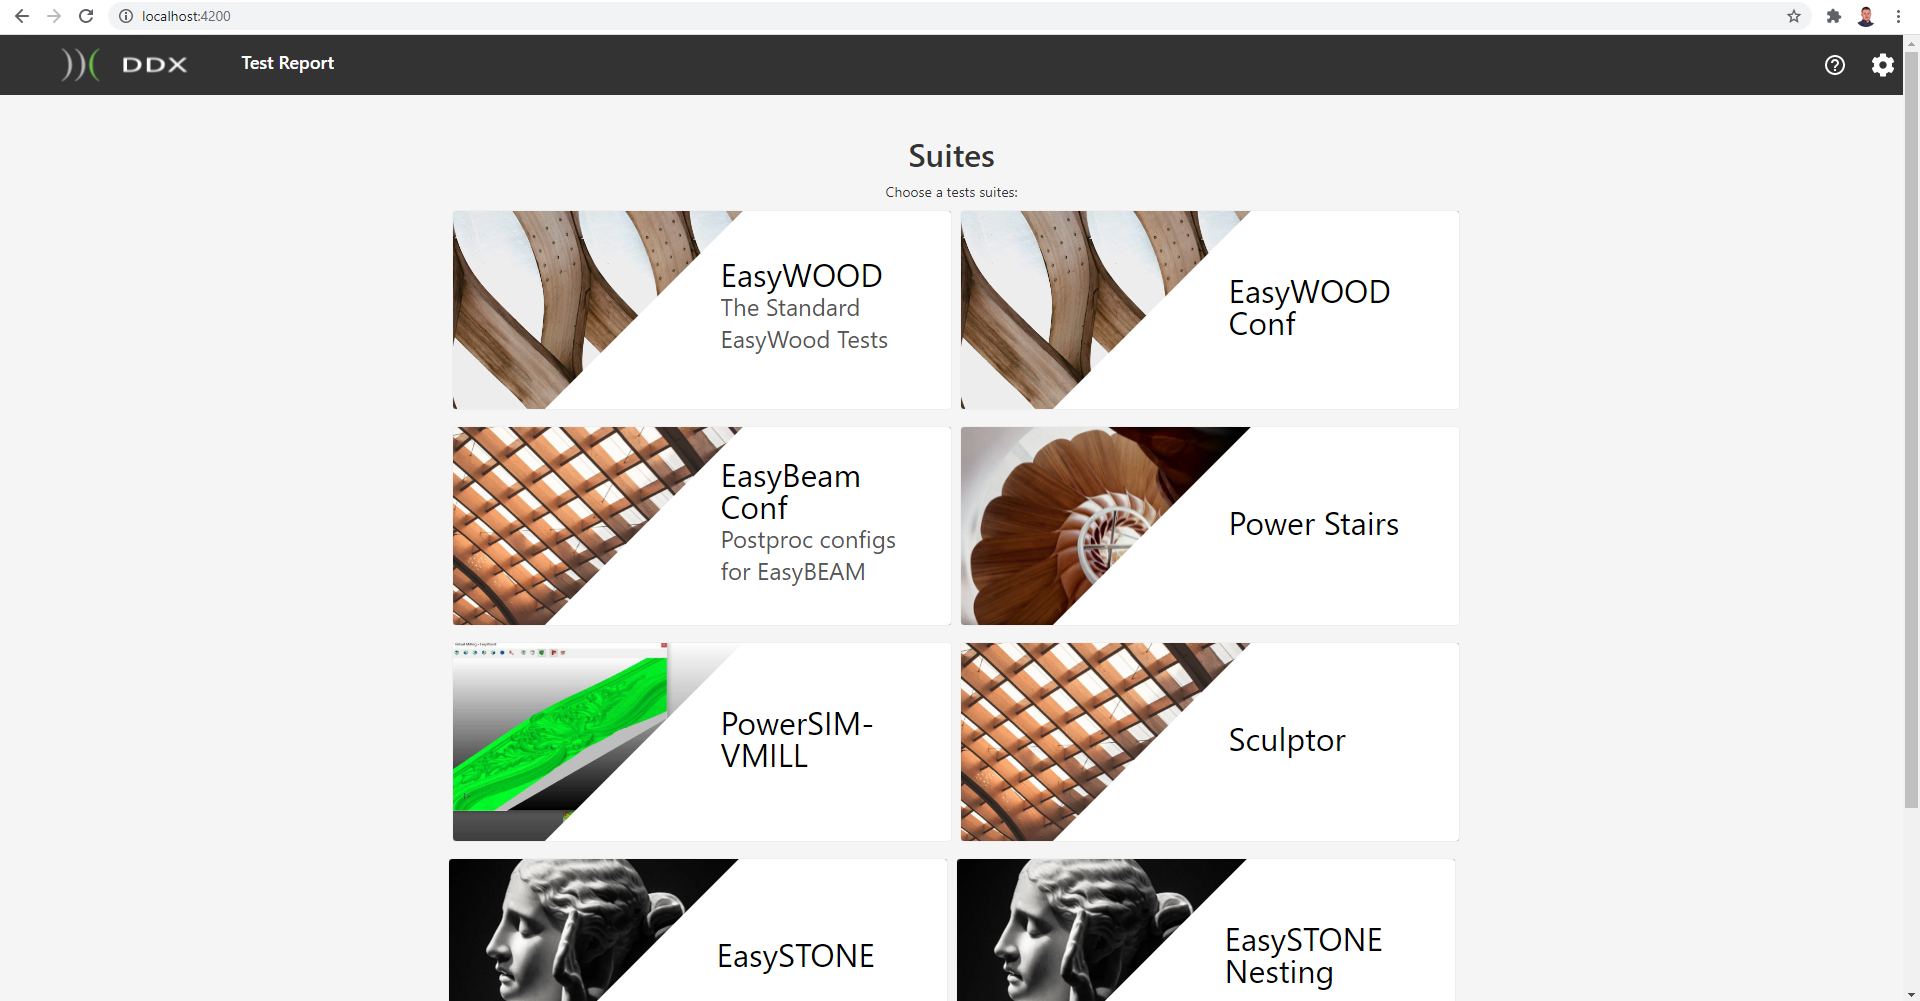
\includegraphics[width=\textwidth]{images/homepage.png}
        \caption{La pagina di home dell'interfaccia web attraverso la quale \'e possibile scegliere quale test suite consultare.}
    \end{figure}
    \section{Angular}
        Angular \'e un framework web che consente di creare applicazioni dinamiche e reattive.    \\
        Questo framework \'e specifico per lo sviluppo di \textit{SPA} (Single Page application).\\
        Una Single Page Application differisce da una applicazione web normale disponendo di una sola pagina e renderizzando dinamicamente i singoli componenti HTML in base allo stato dell'applicazione.\\
        Il rendering dinamico consente una maggiore fluidità nel cambiamento di pagina, non avendo l'overload di richiedere la risorsa sulla rete.\\
        Nonostante le SPA consistano in un solo file HTML hanno comunque la possibililtà di visualizzare documenti specifici in base al loro indirizzo corrente, grazie a un sistema chiamato \textit{Routing}. \\
        \subsection{Scelta dell'utilizzo}
            \'E stato scelto di usare Angular, perchè è un framework completo supportato da Google
            ed \'e già stato usato precedentemente per lo sviluppo di altri applicativi.
            
            Angular ha una struttura a componenti ovvero basici elementi grafici con una singola responsabilità che composti tra loro formano componenti più avanzati e la completa applicazione.
            Questo stile strutturale consente il riuso del codice, per esempio, un componente sviluppato precedentemente consente
            di renderizzare un file CAD proprietario all'interno della pagina web.
        
        \subsection{Typescript}
            Un altro motivo per la scelta di Angular è \href{https://www.typescriptlang.org}{Typescript}.
            Typescript è un \textit{superset di javascript} cioè un'estensione che ne ingloba tutte le funzionalità e ne aggiunge altre.
            La sua peculiarità principale è l'aggiunta di uno step di compilazione che favorisce il controllo della correttezza del codice attraverso una tipizzazione statica.
    \section{Funzionalità}
        La prima responsabilità dell'interfaccia web \'e rendere i test fruibili graficamente.
        Ogni test \'e rappresentato da una scheda (in gergo \textit{card}) che contiene una lista di reference con un indicatore grafico del loro stato.
        \begin{figure}[h]
            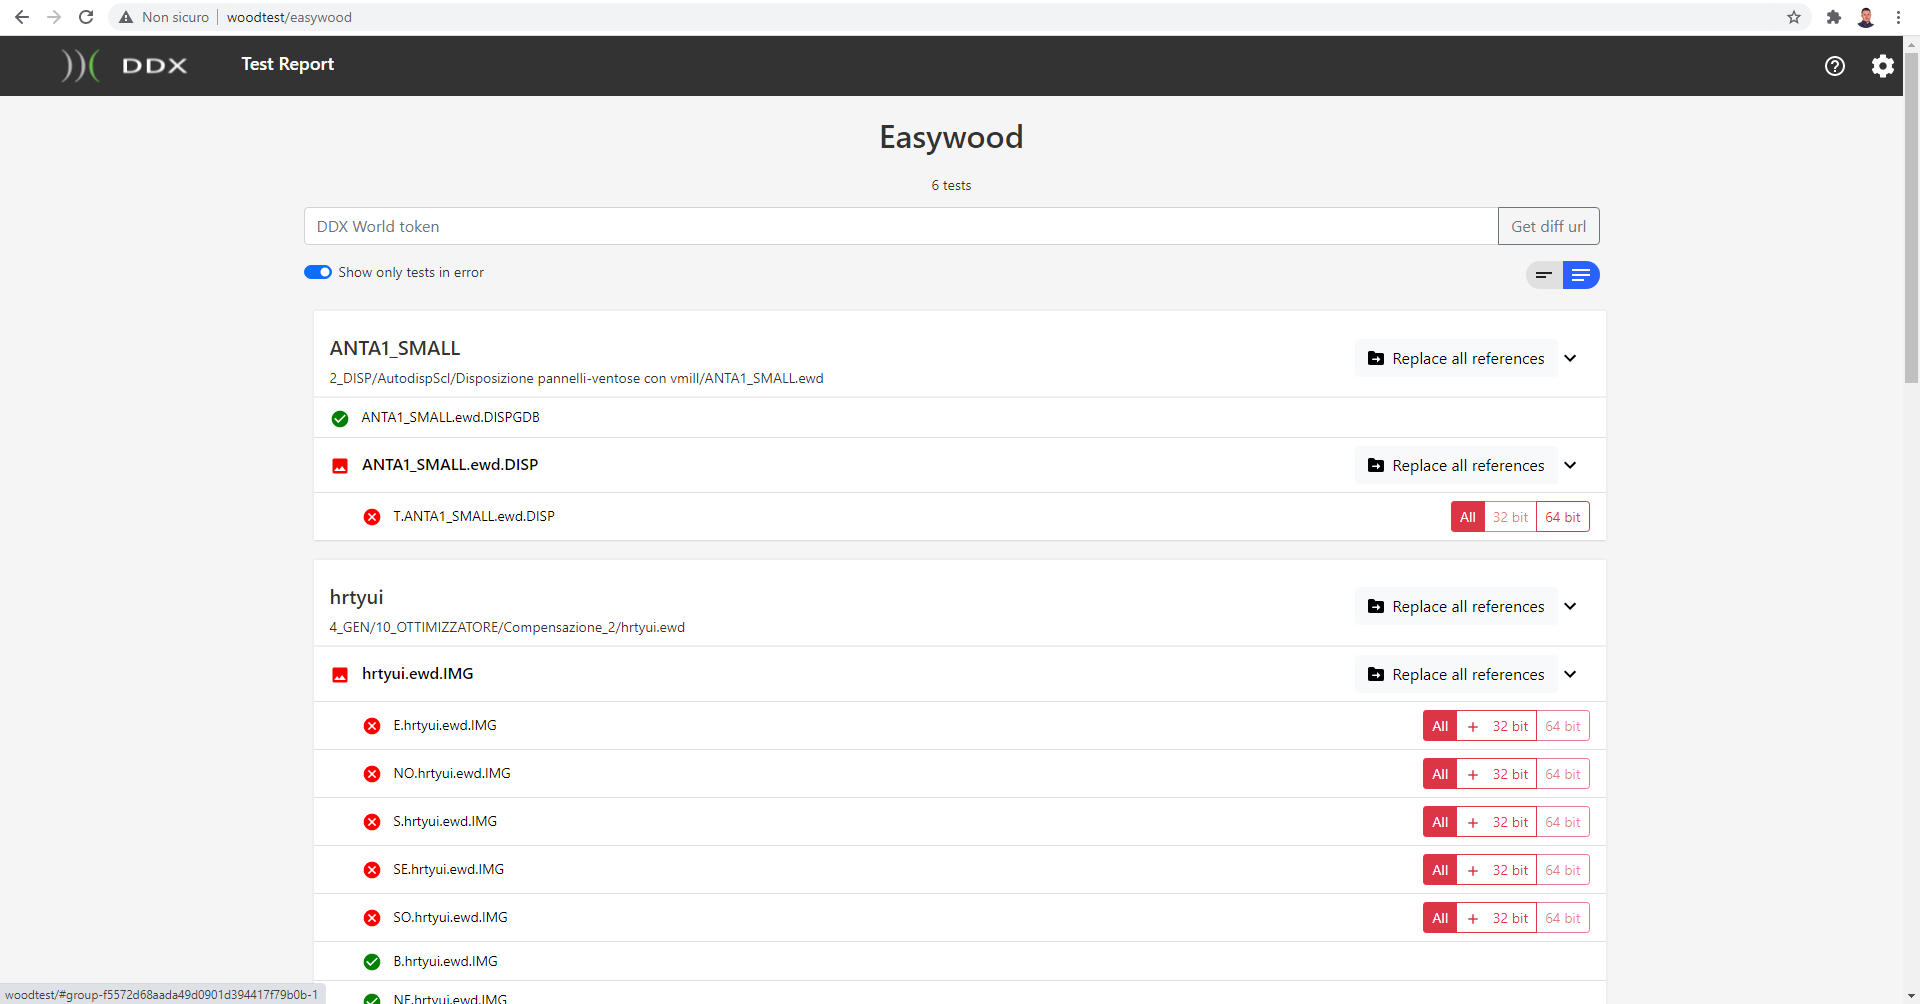
\includegraphics[width=\textwidth]{images/page.png}
            \caption{Un esempio di visualizzazione di test}
        \end{figure}
        \subsection{visualizzazione dei test}        
            Uno scopo del report \'e rendere pi\'u facile individuare i test in errore.
            \'E perci\'o possibile filtrare i test in base al loro stato rendendo visualizzabili solo quelli con almeno una reference differente.
            Lo sviluppatore pu\'o anche nascondere le reference corrette all'interno di una card.\\
            Un ulteriore modo per togliere un test dalla vista \'e l'operazione di \textit{collapse}: essa consente di nascondere tutte le reference lasciando solamente il nome del test.
            Con una specifica pagina di configurazione si pu\'o personalizzare il comportamento del programma in modo che tutte le card vengano collassate all'avvio dell'applicazione.
            
            \begin{figure}[h]
                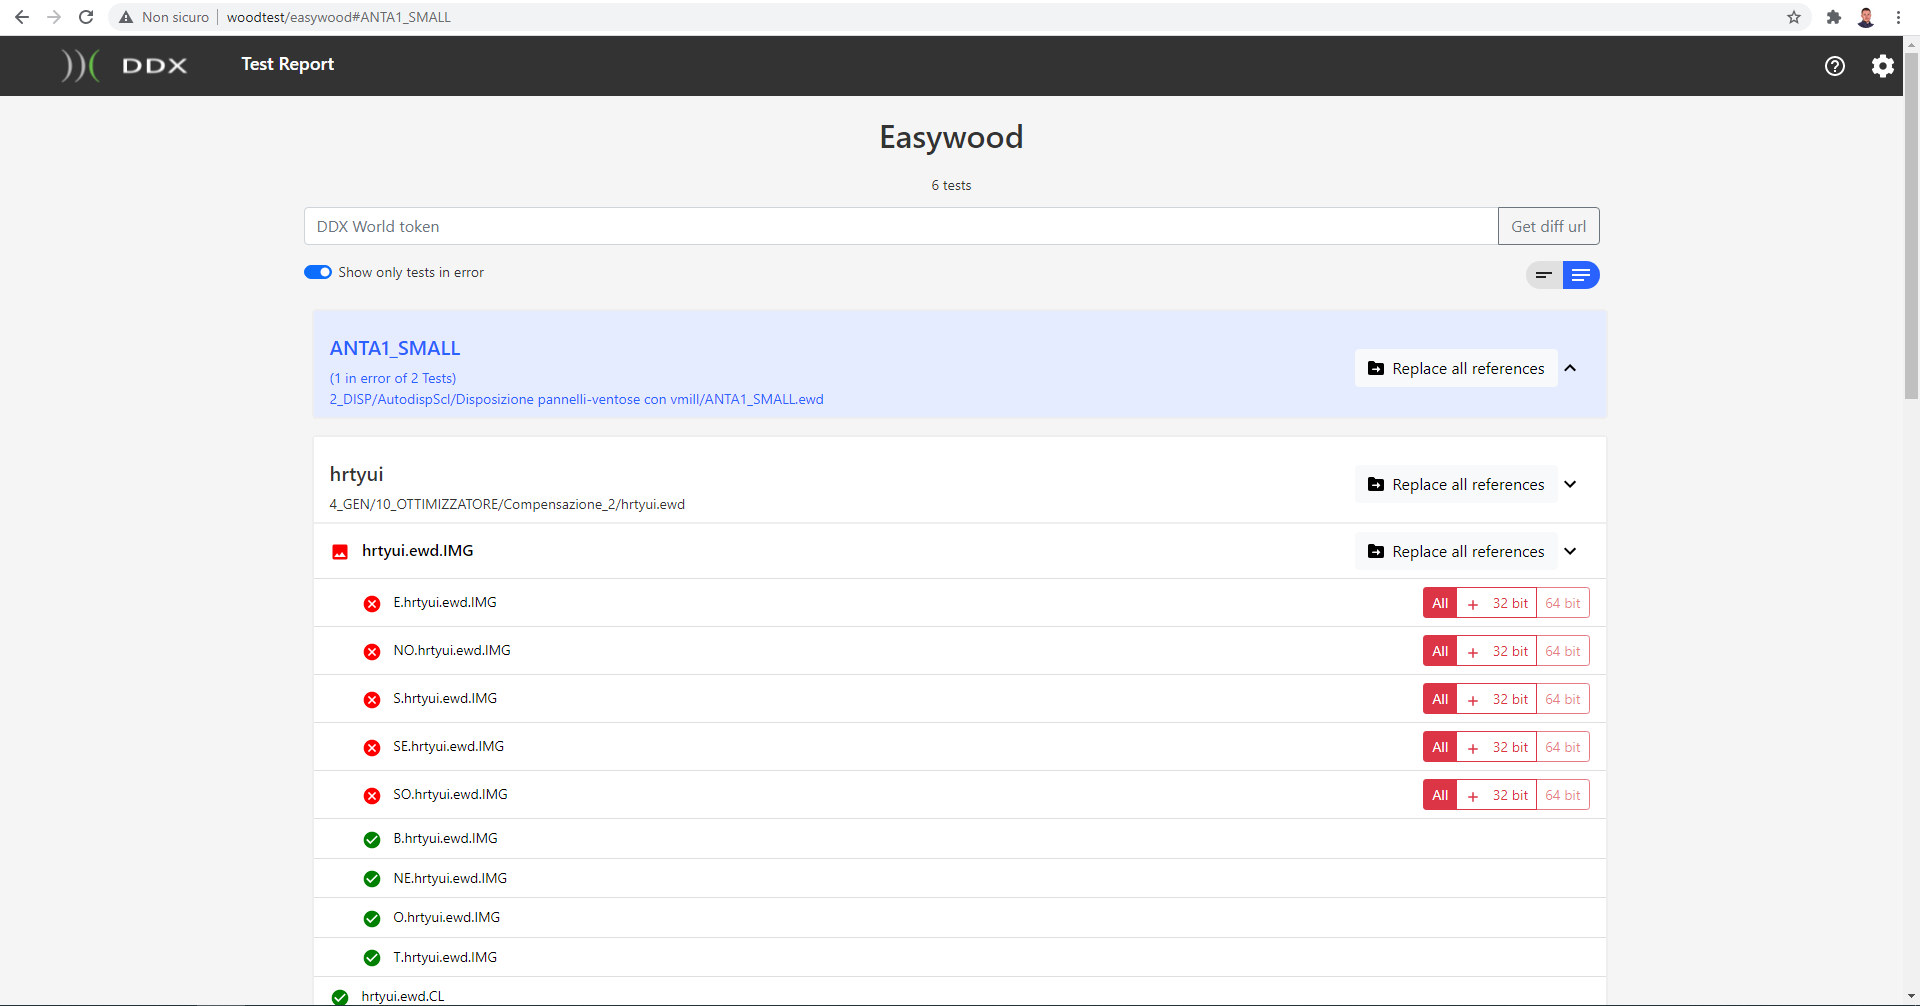
\includegraphics[width=\textwidth]{images/collpapsed.png}
                \caption{Un test in stato \textit{collapsed}}
            \end{figure}
            
            \subsection{Gestione interattiva dei file sovvrascritti}
            L'iter di modifica di un test consiste nel: 
            \begin{itemize}
                \item Confronto di un oracolo con il suo risultato in errore
                \item Aggiunta delle azioni in un area predisposta
                \item Creazione di un commit
            \end{itemize}      
            Il sistema tiene traccia delle azioni effettuate perchè esse non sono effettive e condivise in rete fino a quando non viene creato un commit.
            L'interfaccia web dispone una sezione per salvare le azioni e committarle.
            In un area specifica vengono visualizzate tutte le azioni, che possono essere annullate o definitivamente registrate.
            \subsection{Navigazione}
                \'E disponibile un metodo di navigazione per aumentare l'usabilità dell'applicazione.
                Durante la navigazione è possibile rendere un test \textit{focussed} e effettuare operazioni su esso usando delle scorciatoie da tastiera.\\
                Usando il tasto \textbf{C} E' possibile rendere il test \textit{collapsed} o usando \textbf{S} mettere tutte le sue reference in area di stage.\\ 
                Nello stesso modo si puo spostare il focus della navigazione sul prossimo elemento o su quello precedente, rispettivamente con \textbf{N}(NEXT) o \textbf{B}(BACK).
                Quando il focus si sposta su un nuovo test viene effettuata un operazione di scroll per includerlo nella parte visibile della pagina.
                Lo stato della navigazione viene descritto nell'URL, scrivendo il nome dell'elemento in focus nella sezione denominata \textit{fragment}.\\
                Se la pagina viene richiesta con un fragment già impostato, in fase di rendering dei tests viene posto il focus automaticamente sul test con quel nome (in questo modo sar\'a visualizzabile gi\'a al caricamento della pagina).\\
                La gestione dei fragment rende condivisibile una risorsa primaria dell'applicazione quale il test indirizzandolo tramite un URL, come voluto dalla filosofia web. 
            
            \begin{figure}[h]
                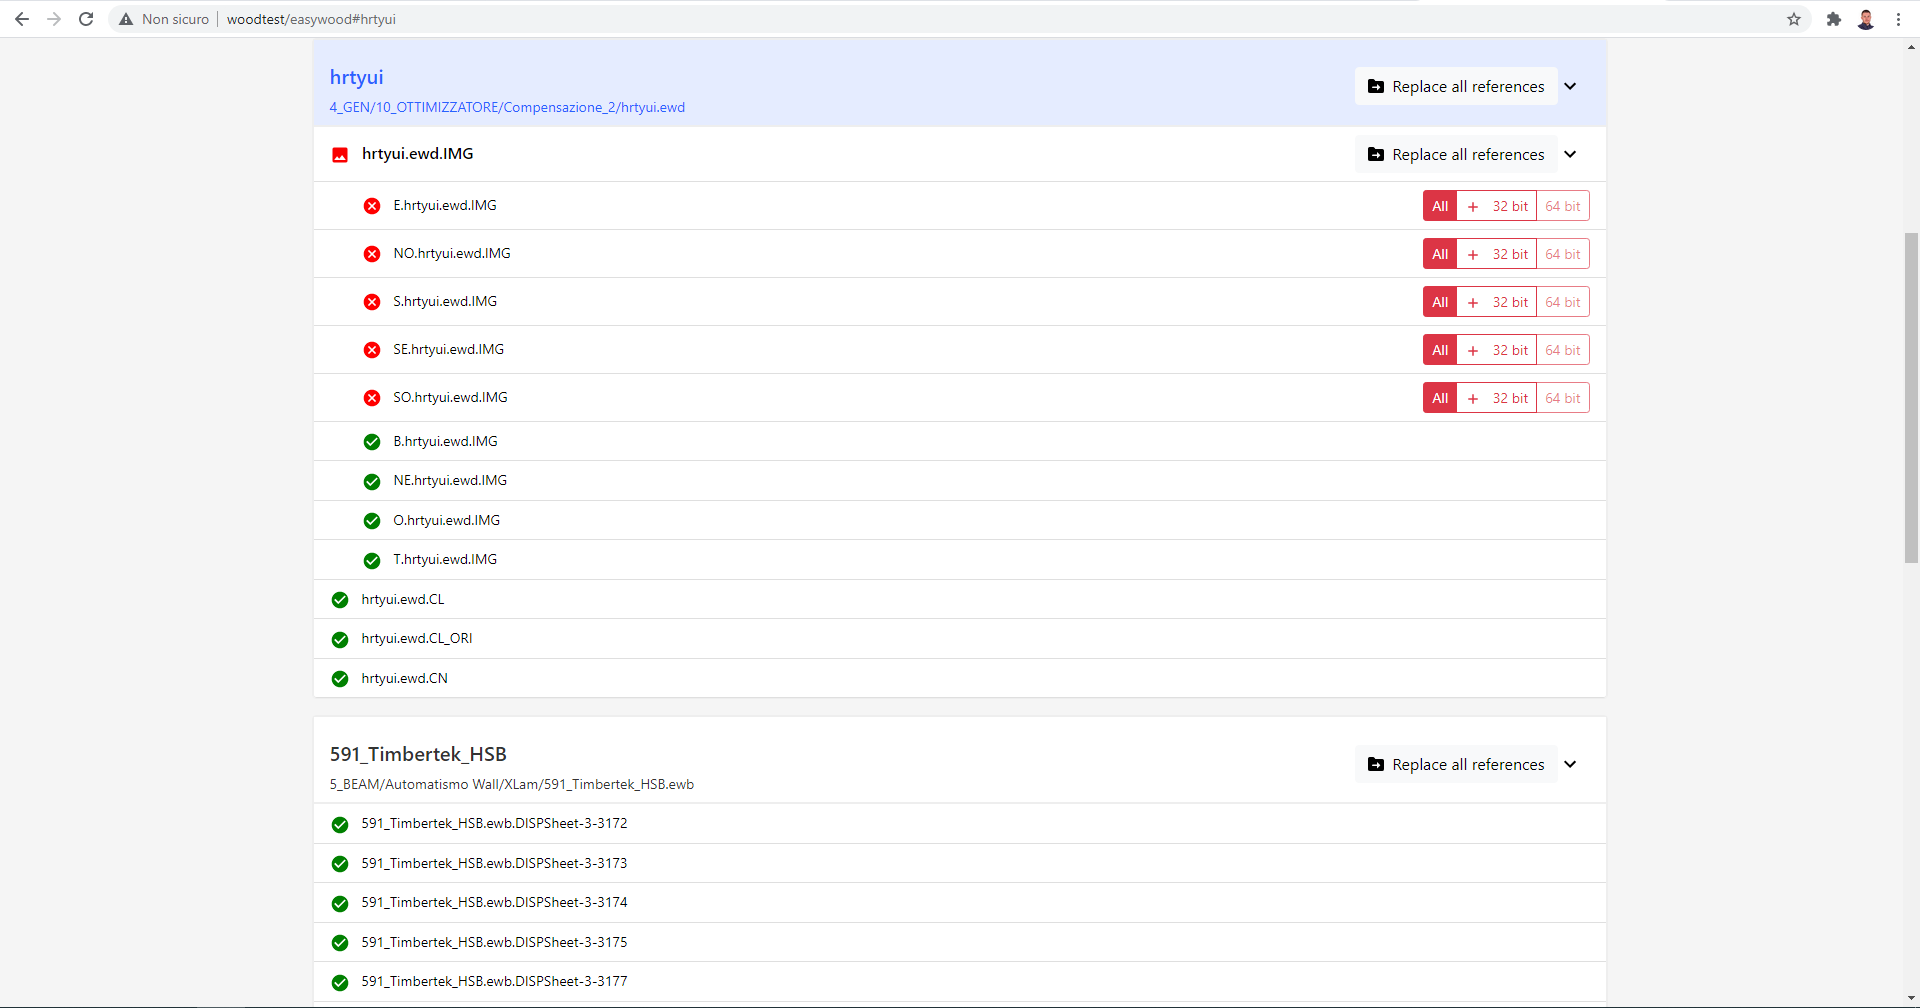
\includegraphics[width=\textwidth]{images/active.png}
                \caption{Un test in stato di focus. La sua scheda relativa viene evidenziata e l'url della pagina viene modificato includendo il nome della risorsa.}
            \end{figure}
            \section{Interazione con gli altri tool aziendali}
                La consultazione delle differenze viene delegata a un tool aziendale già sviluppato in precedenza, denominato \textit{Differ}.
                Anch'esso \'e un tool web quindi questa integrazione avviene  costruendo un URI per navigare nella pagina successiva.
                Il processo di esecuzione dei test di occupa di salvare i risultati di ogni sessione di test e rendere i risultati disponibili tramite Differ mantenendo dunque una cronologia.
                Il report in oggetto, invece produce un interfaccia in tempo reale basata lo stato del server.
                Per sincronizzare lo stato tra i due sistemi \'e necessario recuperare l'ultima sessione di test eseguita e, per ogni reference, creare un url che associ il test con le sue differenze.